










\section{Introduction}

% Motivate importance of field
%           Deep learning has revolutionized a lot of fields (specifically seq to seq) 
%           Mathematical Reasoning is ripe for the same type of revolution 
%               One sentence explanation of mathematical reasoning 
Deep learning, and more recently the advent of sequence to sequence models have notably raised bar on benchmarks in a wide range of 
areas where humans excel. Some of these include visual reasoning (cite), understanding language (cite), and playing games like Chess or Go (cite). \\ 

\begin{figure}[hbt!]
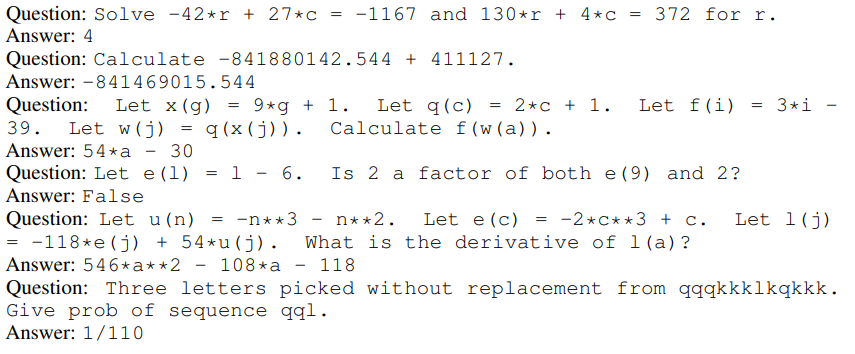
\includegraphics[width=12cm]{images/math_examples_bunch.PNG}
\centering
\caption{A sample set of math questions drawn from the novel dataset. This figure was taken directly from the original Saxton et al. paper \supercite{DBLP:journals/corr/abs-1904-01557}}
\label{fig:mathexamples}
\end{figure}

However a separate type of reasoning that is used just as much by humans as the others--mathematical reasoning--is still relatively unexplored in the machine learning literature (cite) . This type of reasoning involves using  wide array of cognitive skills and learned generalization ability to manipulate symbols and formal systems via logical rules. If the same techniques that were successful on other types of reasoning could be applied to mathematical reasoning we might be able to learn a lot about how this type of reasoning works and also drastically improve the performance computers have on problems that require this. \\ 

% Explain the contributions of Saxton et al. 
%           New Dataset
%           Sequence to sequence  Model Performance 
Towards this goal, the authors of Saxton et al. \supercite{DBLP:journals/corr/abs-1904-01557}  provide two key contributions. They, 

\begin{itemize}
   \item Introduce a novel and robust dataset of mathematical tasks including problems from algebra, probability, calculus, etc.
   \item Conduct initial deep learning experiments by evaluating multiple sequence to sequence models on their dataset 
\end{itemize}

Diving more into the first contribution, the dataset the authors introduce contains a variety of mathematical problems in a sequence to sequence format. In additional to these pre-generated questions, they also provide code that allows one to generate even more mathematics problems with a similar structure to those that were pre-generated. A set of example mathematics problems in this dataset along with their solutions can been seen in Figure ~\ref{fig:mathexamples}. They hope that this curated set of mathematics problems will eventually serve as a benchmark for models trying to demonstrate exceptional mathematical reasoning.  \\


For their second contribution, they train a modern transformer network and a variety of LSTM networks \supercite{hochreiter1997long} to demonstrate how sequence to sequence models perform on their dataset. They find that performance is good many different types of problem but definitely not all. They also find that in general, the trained sequence to sequence models do not achieve good generalization metrics across different problem types.  \\ 

% Stating what we are reproducing and why we think the reproduction is valuable 

In this work, we reproduce the paper of Saxton et al.\supercite{DBLP:journals/corr/abs-1904-01557}. We detail our methodology and challenges (Section 0.0 ), test model performance on the released interpolation and extrapolation mathematics datasets (Section 0.0), compare the published results to our findings (Section 0.0),  and release an ablation study (Section 0.0).  Our source code and model files are available on GitHub [1].


\section{Related Work}

% Related Work from Saxton Paper (2 paragraphs)
There have been a couple studies prior to Saxton et al. \supercite{DBLP:journals/corr/abs-1904-01557} exploring mathematical reasoning and discrete reasoning in general. For example, work has been done to solve addition and multiplication tasks using variations of convolutions neural networks that achieve good generalization properties \supercite{kaiser2015neural}. Other research has pursued "neural equivalence networks" for learning tasks related to symbolic algebra and boolean expressions \supercite{allamanis2017learning}. Finally there has also been progress by Evan et al. using tree-structured neural networks to understand logical entailment \supercite{evans2018neural}.   \\

Furthermore, past research efforts have gone into solving algebraic word problems. These types of problems involve formulating algebraic equations into a sentence or paragraph which forces the student to reassemble and solve the equation uses the sentences logic directly. From the attention given to solving these, many useful datasets have arisen. Examples of datasets include those created by the Allen Institute for AI, Kushman et al. \supercite{kushman2014learning}, Huang et al. \supercite{huang2016well},  Upadhyay \& Chang \supercite{upadhyay2016annotating}, Wang et al. \supercite{wang2017deep}, and Ling et al. \supercite{ling2017program}. These datasets all vary heavily but there is a general trend toward including more narrow types of problems and providing supervised data about how to reason about specific problem types.  \\


%Contrast Saxton et al. with relevant work and explain the space in which it was published 
In contrast to these studies, Saxton et al. \supercite{DBLP:journals/corr/abs-1904-01557} carves out its niche by providing a novel dataset of mathematics tasks ranging from algebra, arithmetic, and probability to calculus and number theory. This dataset focus directly on the mathematics reasoning rather the underlying linguistic interpretation used within solving word problems and also includes more variety in the areas of mathematics it covers. The paper authors purposely try to isolate the mathematical reasoning from the linguistic interpretation in order to only measure that capacity. \\

% Related Work that has happened since the release of Saxton Paper (1 paragraph) 
More related work has emerged after the publication of Saxton et al.\supercite{DBLP:journals/corr/abs-1904-01557} that is related in spirit. For example, Lample \& Charton \supercite{lample2019deep} use deep learning to solve more elaborate mathematical tasks such as symbolic integration and differential equations with surprising success.  Additionally, Wallace et al. \supercite{wallace2019nlp} investigated how well language models embed numbers finding that many common language embeddings excel on a variety of numeracy tasks. This supports the idea that language embedding currently capture numeracy to a high degree. \\


\section{Experimental Methodology} \\
In order to validate the original authors’ results, we attempted to replicate the settings of the described models and test their performance on the interpolate and extrapolate mathematics datatsets. The models chosen were the vanilla Transformer\supercite{vaswani2017attention}, simple LSTM, an attentional LSTM. We omitted the relational memory core and non-bidirectional LSTM encoder models because their results seemed inline with the other models and they were not included in the original paper’s figures 4 and 5. The authors did not publish the training code, but the model architecture and training process was well-described. The authors were responsive to our questions over email for further details. In this section, we describe our implementation and clarify our decisions. 

\subsection{Implementation Details} \\

We replicated the models using PyTorch\supercite{paszke2019pytorch}. Our implementations were based off popular open-sourced implementations\supercite{nlp-tutorial}\supercite{pytorch_math_dataset}\supercite{attention-is-all-you-need}. Although the original paper does not reference a neural network framework, the authors responded to us that they used the library Tensor2Tensor\supercite{vaswani2018tensor2tensor} for their Transformer and a custom Sonnet\supercite{sonnet} library implementation for the LSTMs.\\

We trained the models according to the hyperparameters set in the paper: a batch size of 1024, Adam optimizer with learning rate of $6 \times 10^{-4}$, betas 0.9 - 0.995, and eps of 1e-9 [USE LATEX NOTATION], no dropout, and absolute gradient clipping of 0.1. The authors write that the hyperparameters were found via sweep. The questions were fed to the models as sequences of characters and training was stopped at 500k batches.\\

The Transformer was configured with an embedding size of $d_{model} = 512$, with h = 8 attentional heads. Key and value sizes were dk = dv = dmodel/h = 64. Each model layer has an intermediate representation with dimension dff = 2048. The "Simple LSTM" used a hidden size of 2048. The "Attentional LSTM” used an encoder of 512 hidden units and decoding LSTM with 2048 hidden units. The LSTMs were also fed zero input 15 times before outputting an answer, to allow for additional computational steps. \\

Specific care in our reproduction was put into deterministically conducting training and benchmarking. We used fixed seeds for shuffling data, Numpy, and PyTorch. PyTorch and cudnn were set to deterministic mode. We tested and confirmed that running the training code multiple times on the same machine results in identical learning trajectories. \\

We include two ablation studies: one with a batch size of 128 and another with a learning rate of 6e-6. \\

Our open-source repository\supercite{hs-math-nlp} includes the training and benchmarking code. The 112 million datapoint, 7.8GB dataset is downloaded from the public site provided by by the authors\supercite{dataset}. Instructions for installation and running both training and benchmarking are in the readme. Training logs are viewable with TensorBoard\supercite{tensorboard}. Checkpoint model files are available in the repository's releases section, including each of the 4 completed epochs, the final 500k batch version, and our ablation study. \\

\subsection{System and Cost} \\

For future reproducibility efforts, we describe our compute for running the experiments. We deployed to Google Cloud Platform region us-central1-b. Our experiments utilized preemptible (also known as spot) virtual machine instances, deterministic shuffling, and mid-epoch checkpointing, which reduced costs by about two thirds. \\

Total cost for training the Transformer model in region us-central1 was approximately \$1350. 97GB of VRAM was required to support a batch size of 1024, so 8 NVIDIA V100s were attached to a n1-standard-8 virtual machine. Training took approximately [32 hours] for 500k batches. \\



\section{Results}

\subsection{Transformer Performance}

%% Brief Explanation of performance in words

After training, our transformer achieved ... The puts our model .... with regard to the original papers model. A side to side performance comparison 

%%% Have figure showing the accuracy of our transformer vs. their transformer of average of interpolation/extrapolation performances

\begin{figure}[h]
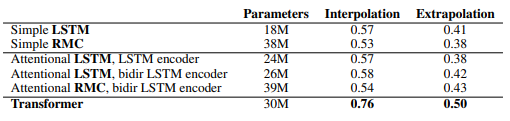
\includegraphics[width=8cm]{images/test_image.PNG}
\centering
\caption{This figure shows the comparison of our transformer vs. the transformer by the original authors}

\end{figure}

\begin{figure}[h]
\centering
\begin{tabular}{SSSSSSSS} 
    {} & {\textbf{Interpolation}} & {} & {\textbf{Extrapolation}} & {} \\ \midrule
    \makecell{\textbf{Transformer} \\ \textbf{Transformer} (ours) } & \makecell{0.76 \\ 42} & 40 \% & \makecell{0.50 \\ 43} & 40 \%  \\ \midrule
    \makecell{Attentional \textbf{LSTM} \\ Attentional \textbf{LSTM} (ours) } & \makecell{0.54 \\ 42} & 40 \% & \makecell{0.43 \\ 43} & 40 \%  \\ \midrule
    \makecell{Regular \textbf{LSTM} \\ Regular \textbf{LSTM} (ours) } & \makecell{0.57 \\ 42} & 40 \% & \makecell{0.41 \\ 43} & 40 \%  \\ \bottomrule
\end{tabular}
\caption{Table of Model Performances}
\end{figure}


% \begin{figure}[h]
% \centering
% \begin{tabular}{SSSSSSSS} 
%     {} & {\textbf{Interpolation}} & {\textbf{Extrapolation}} \\ \midrule
%     \textbf{Transformer}  & 16.128 & +8.872  \\
%     \textbf{Transformer} (ours)   & 3.442  & -2.509  \\ \midrule
%     Attentional \textbf{LSTM}  & 1.29   & +0.099 \\
%     Attentional \textbf{LSTM} (ours)  & 0.483  & -0.183 \\ \midrule
%     Regular \textbf{LSTM}  & 0.624  & +0.365 \\ 
%     Regular \textbf{LSTM} (ours)  & 0.641  & -0.466  \\ \bottomrule
% \end{tabular}
% \caption{Table of Model Performances}
% \end{figure}

\subsection{LSTM Performance}

The results for both the attentional and regular LSTM showed ... This puts them ... Figure ... shows 

\begin{figure}
\centering
\begin{subfigure}{\textwidth}
  \centering
  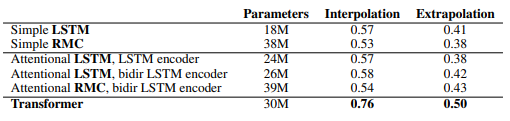
\includegraphics[width=3cm]{images/test_image.PNG}
  \label{fig:sub1}
\end{subfigure}%
\begin{subfigure}{\textwidth}
  \centering
  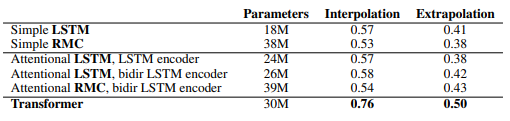
\includegraphics[width=3cm]{images/test_image.PNG}
  \label{fig:sub2}
\end{subfigure}
\caption{This figure shows a performance comparison of our attentional and regular LSTMs versus the respective LSTMs trained in the original paper}
\label{fig:test}
\end{figure}


\section{Analysis and Discussion}


\section{Conclusion}
